\documentclass[sigconf]{acmart}

\usepackage{graphicx}
\usepackage{amssymb}
\usepackage{amsmath}
\DeclareMathOperator*{\argmin}{arg\,min}
\linespread{1.4}

\settopmatter{printacmref=false} % Removes citation information below abstract
\renewcommand\footnotetextcopyrightpermission[1]{} % removes footnote with conference information in first column
\pagestyle{plain} % removes running headers

\title{Dynamic Pricing Strategies, Result Team 4}
\author {Jonas Bounama, Tim Oesterreich, Robert Stark}
\date{}
% %
% %%%%%%%%%%%%%%%%% END OF PREAMBLE %%%%%%%%%%%%%%%%
% %

\begin{document}

\begin{abstract}
Bartering on street markets is still a nice family activity for sunny Sundays. People can go there and catch a bargain for all kinds of products. Usually the merchant makes a profit, even if he reduces the price by 30\%. On the Internet the price war is not that friendly. Here, people make their living selling products for the best possible value. To maximize their profits, these online merchants use dynamic pricing strategies. By analyzing their opponents, they are able to set prices that are just the right amount, so that a potential customer buys their product over the product of a different merchant. The best thing is that these strategies run completely autonomous. The following pages will explain how this is done and present our own implementation.
\end{abstract}
\maketitle

\section*{Introduction}
In the scope of the masters seminar ``Dynamic Pricing Strategies'' at Hasso-Plattner-Institute, we developed strategies to predict profitable prices for a real world market situations. For that we tried out different machine learning strategies, making them challenge more simple, rule-based strategies, such as ``always have the cheapest price'' or ``use random prices''. After realizing, that a lot of other groups in the seminar used very similar approaches, we wanted to see what other solutions we could find. After some research our focus fell on the ``Passive Aggressive Regressor'' and the ``Bayesian Ridge Regressor''. In this paper these two regression algorithms are explained, compared and finally tested on a simulation platform.

\section*{Passive Aggressive Regression}
The Passive Aggressive Regression is part of a family of binary classifications.

\subsection*{Binary Classifications}
A binary classifier tries to predict if the value of an instance is 1 or -1. This is done using a prediction function that calculates a value in range [-1, 1] based on a set of input values, which is compared to the actual value. The resulting deviation is used to adapt future predictions.\\
This procedure is applied multiple times. We will call one of these runs \emph{t}.\\
The set of input values is a vector $\mathbb{R}^n$ and is defined as $x_t$. For each $x_t$ a $y_t\in \{+1, -1\}$ is expected. A pair $(x_t, y_t)$ is called example.\\
Furthermore, a binary classifier has a weight factor $w\in \mathbb{R}^n$ with values $sign(w*x)$. The absolute value $|w*x|$ can be interpreted as a trust value for the prediction.
$y_t$($w_t$*$x_t$) defines the margin for each example. If the margin is positive, $sign(w*x)$ equals $y_t$ and the correct value was predicted. The aim is to keep the margin as high as possible, especially not letting is drop below 1.0, so the prediction has a high trust value.\\
If a value less than 1.0 is reached, a loss in form of a hinge-loss function is defined:

\[
  l(w(x,y))=\left\{
  \begin{array}{ll}
    0, & y(w*x)>= 1 \\
    1-y(w*x), & else
  \end{array}\right.
\]

Choosing 1 as threshold for the loss is arbitrary and can have different values. We want to find a weight factor for every point \emph{t}, such that there is as little loss as possible.

\subsection*{Handling the Weight Factor}

The weight factor is initially set to 0 for each point \emph{t}. It is necessary to define modification rules. Three different approaches are available to achieve this.\\
The first approach chooses $w_{t+1}$ so that the following equation is fulfilled:

\begin{center}
$w_{t+1} = \argmin\limits_{w\in \mathbb{R}^n}\frac{1}{2}||w-w_t||^2$ , so that $l(w;(x,y)) = 0$
\end{center}

This also shows the origin of the name `Passive Aggressive Regressor'. The adaption of the weight factor only occurs if a loss happened. In this case an aggressive behavior is chosen. If there is no loss, no change is made, which is called passive behavior.

The adaption itself occurs like this:

\begin{center}
$w_{t+1} = w_{t} + \tau_{t}y_{t}x_{t}$ | $\tau_t = \frac{l_t}{||x_t||^2}$
\end{center}

Due to the aggressive adjustments of the equation, changes of the weights can potentially have a very significant effect on the result. To avoid extreme jumps, another approach is to choose an aggressiveness factor. This factor defines a maximum adaption value. During the fitting of the model, the first approach is chosen. The resulting adaption factor is compared to the aggressiveness factor and the minimum of both is used for further fitting.\\

\begin{center}
$\tau_t = min\{C, \frac{l_t}{||x_t||^2}\}$\\
\end{center}

The third approach aims to avoid hard borders during the adaption. Instead, the aggressiveness factor is used as a relative component that controls the adaption.\\

\begin{center}
$\tau_t = \frac{l_t}{||x_t||^2 + \frac{1}{2C}}$\\
\end{center}

In pseudo code the implementation would look like this:\\

\noindent
\textsc{Input:} aggressiveness parameter C > 0\\
\textsc{Initialize:} $w_1 = (0, ..., 0)$\\
For $t = 1, 2, ...$
\begin{itemize}
  \item receive instance: $x_t \in \mathbb{R}^n$
  \item predict: $y_t = sign(w_t * x_t)$
  \item receive correct label: $y_t \in {-1, +1}$
  \item suffer loss: $l_t = max{0, 1-y_t(w_t * x_1)}$
  \item update:
  \begin{enumerate}
    \item set:\\
      \begin{tabular}{ l  l }
        $\tau_t = \frac{l_t}{||x_t||^2}$ & (PA)\\
        $\tau_t = min\left\{C, \frac{l_t}{||x_t||^2}\right\}$ & (PA-I)\\
        $\tau_t = \frac{l_t}{||x_t||^2 + \frac{1}{2C}}$ & (PA-II)
      \end{tabular}
    \item update: $w_{t+1} = w_t + \tau_t * y_t * x_t$
  \end{enumerate}
\end{itemize}

\section*{Bayesian Ridge Regression}
This regression also belongs to the family of linear regressions. That means, given a vector of attributes $x_i \in \mathbb{R}^n$ an attribute $y_i$ should be predicted. Similarly to the passive aggressive regression, we want to find a weight factor $w\in \mathbb{R}^n$. A naive linear regression algorithm assumes that there is a model that is able to exactly describe a given data point. However, this usually is not right as there are at least random deviations.\\
A Bayesian model assumes that the deviations occur normally distributed, as seen in figure \ref{img:bayes_func}.\\

\begin{figure}
  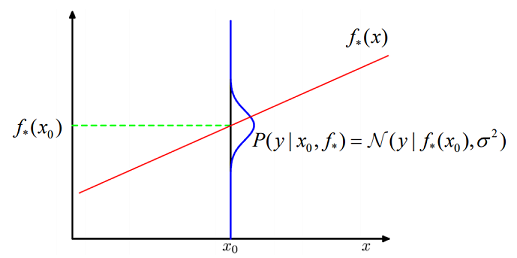
\includegraphics[width=\columnwidth]{pictures/Bayer_funktion.png}
  \caption{Deviations in the model}
  \label{img:bayes_func}
\end{figure}

The resulting attribute can be described with the following formula:
\begin{center}
$y = f_*(x) + \varepsilon$ | $\varepsilon ~ N(\varepsilon|0,\sigma^2)$
\end{center}

$\sigma$ is the parameter that represents the amount of the deviation.\\
Observing the weight factor, you can see an a-priori distribution. Bayes' theorem and this distribution is used to calculate the a-posteriori distribution. The a-posteriori distribution represents knowledge that includes prior knowledge. This behavior is implemented in Bayesian regression. The Prior Function is used to create this distribution. The function has the following structure:
\begin{center}
$y* = arg max_{y}P(y|x,L)$
\end{center}

$L$ represents the likelihood function.

\section*{Scoring}
To find out how well a chosen model is able to classify given data, multiple scoring possibilities are available. These algorithms try to calculate a numerical value that enables an objective comparison of different models.

\subsection*{Akaike Information criterion}
The \textbf{Akaike Information criterion} (AIC) measures the relative quality of models. Given a set of models and a set of data, AIC calculates a score that compares the quality of a model to each other model. The best model is the one that minimizes the \textbf{Kullback-Leibler divergence} between itself and the truth. The Kullback-Leibler divergence is a way to measure the divergence from one probability distribution to a second one.\\
\newpage
The AIC is defined as
\begin{center}
$$AIC = -2 * (ln(likelihood)) + 2*K$$
\end{center}
\textit{likelihood} defines the probability of the data given a model. \textit{K} is the number of parameters of the model. As the AIC compares statistical models relative to each other, it is usually shown as $\Delta AIC$. So the best model has a $\Delta AIC$ of zero.

\subsection*{Likelihood function}
The likelihood function estimates the chance that a given model is true. It can be understood as the opposite of a probability function. Assuming the scenario that we want to sell a book with condition $x$ in a given market situation with $n$ other merchants, the probability function would tell us how likely it is, that we will sell this book for a given price. The likelihood function in contrast estimates how likely it is, that a model that predicted a certain probability of selling that book with all its parameters, fits the reality. So maximizing this value is a procedure to determine the best model parameters that fit the given data. It is also a way to compare multiple models to determine which has the best fit to the data, which is why the likelihood function is used for AIC calculation.\\
The general formula for the likelihood function is:
\begin{center}
$$L(\theta | x_i) = \prod f(x_i|\theta)$$
\end{center}
$\theta$ is a set of parameters given to the model. So the likelihood function is the product of the probabilities of observing the data $x_1, x_2, ..., x_n$ given that they come from a distribution with parameters $\theta$. Essentially, $\theta$ is the factor that should be optimized, however maximizing the likelihood function itself is a difficult and expensive task.\\
To actually determine the best model, the \textit{log-likelihood} function is maximized. The logarithm turns the product into a sum:
\begin{center}
$$ln\ L(\theta | x_i) = \sum ln f(x_i|\theta)$$
\end{center}

This reformatting results in equally comparable results, but makes computations easier.\\
For our demand learning, we used the binominal loglikelihood.
\begin{center}
$$f(x_i|\theta) = \theta\ ln\ x_i + (n - \theta)*ln(1 - x_i)\ |\ n = samplesize$$
\end{center}

\subsection*{McFadden pseudo-$R^2$}
The McFadden pseudo-$R^2$ is a scoring algorithm that estimates the goodness of the explanatory variables of a model. It is defined as\\
\begin{center}
$$R^2_{McFadden} = 1 - \frac{log(L_c)}{log(L_{null})}$$
\end{center}
Where $L_c$ is the likelihood value from the current model and $L_{null}$ is the corresponding value from the null model. So the model that only has an intercept as explanatory variable, so it predicts every individual in the data with the same probability of success and does not take its environment into account at all.\\
That means that a model that has very little predictive ability will have a likelihood close to the likelihood of the null model. Therefore the ratio of the likelihoods will be close to 1 and the McFadden pseudo-$R^2$ will be close to 0.\\
Assuming our model explains almost all of the variation in the outcome, the likelihood of this model will be close to 1. $log(1)$ equals 0, which results in the fraction being close to 0 and the McFadden pseudo-$R^2$ will be close to 1.\\
A high McFadden pseudo-$R^2$ value therefore means that a model is very good at explaining variations in the data. As this is usually not a reasonable assumption for most models, the score will most of the time be much smaller. Values from 0.2 to 0.4 are interpreted as an excellent model fit.

\section*{Hyperparameter Tuning}
Most machine learning models have static variables called \textit{Hyperparameters}. Those are parameters that are fixed prior to the learning process. Other parameters are determined through training. Hyperparameters in our approaches are, for Bayesian ridge regression:\\
\begin{itemize}
  \item $alpha\_1$: shape parameter for the distribution over the alpha parameter
  \item $alpha\_2$: rate parameter for the distribution over the alpha parameter
  \item $lambda\_1$: shape paramter for the distribution over the lambda parameter
  \item $lambda\_2$: rate parameter for the distribution over the lambda parameter
\end{itemize}

The alpha and lambda parameters themselves are not hyperparameters, but are controlled by the corresponding ones. They are distributions that determine the precision of the Gaussian distribution of the model.\\
It is usually not obvious which values are ideal for these hyperparameters. The best way find out a good value for them is automatized hyperparameter tuning. The concept is to find a way to minimize a loss function over the model.\\
Our approach is to take our model after a first training pass over the data with its default hyperparameter values. Then we use cross validation over a test data set. Cross validation is a way to evaluate how the model performs on an independent data set, i.e. a data set that was not used for training at all. During this cross validation we calculate the negative McFadden pseudo-$R^2$ of the classification. As the algorithm we use minimizes the score, calculating a negative value means that the smallest result actually yields the best fitting model.\\
Our minimization algorithm does this cross-validation a number of times. Using a Gaussian distribution it tries to change the hyperparameters so, that an optimal value is achieved.

\section*{Feature Selection}
Another important optimization technique is feature selection. A model can depend on a very large amount of features. Actually, every possible data point that has some kind of connection to the data can be used to fit a model. However, a model should always generalize over a given data set. A reason why many models don't perform well is over-fitting. If a model is given all relevant features in a training set and as much time as it wants, it will eventually be able to classify the vast majority of data correctly. If it is given a different data set to classify, this performance might drop significantly. This happens when a model basically memorized the training set.\\
Feature selection can help to avoid this. The aim is to only choose the subset of features that are really relevant. Often features are redundant or not connected to the data at all. For example, the air pressure at the time of a certain sale offer might tell the model whether or not the sale was made, but is not actually correlated to the event.\\
During the training of our models we found out, that the price of a product actually does not have much impact on the performance of the model and might actually decrease the scoring values during cross-validation. Over-fitting is a possibility of this phenomenon.\\
Further reasons for feature selection are general simplification of the model, which can be helpful for understanding the results and possibly manual validation of the model and shorter training times, resulting in a more efficient data fitting.

\section*{Demand Learning Implementations}
We implemented two demand learning strategies. The Passive Aggressive Regressor and Bayesian Ridge Regression. The functionality of both is described in chapter 1. Our implementation uses scikit-learn, a data-analysis library for python. scikit-learn makes it possible to very easily change the model without having to change the code very much. That way all the following steps are valid for both our strategies.\\
Our models require three different data inputs. A training market situation, which will be the data the model tries to fit to, a test market situation for cross validation and a collection of buy offers, which tells the model which data is positive, i.e. a sell, and which is negative. The data has to be provided in csv format, providing at least information about 'amount\_of\_all\_competitors', 'average\_price\_on\_market', 'distance\_to\_cheapest\_competitor',\\
'price\_rank' and 'quality\_rank', as these are the features that provided the best results during manual feature selection.\\
The first step is to aggregate the csv files so, that each entry in the market situation is mapped to an entry from the buy offers. This is done by merging entries with the same timestamp.\\
After bringing the data into a processable format, we can begin training. The data is filtered for our selected features and then normalized. We pass the filtered training data and the corresponding results (sold or not sold) into the model and call its $fit$ function. This sets the internal parameters of the model to values specified by its algorithms.\\
In order to refine this first model, we apply cross-validation and hyperparameter tuning, as described before.

\section*{Merchant Results}
The final results of our training showed that the Passive Aggressive Regressor achieved a McFadden pseudo-$R^2$ of 0.11 and an AIC of 25817, while the Bayesian Ridge Regressor got a score of 0.19 and an AIC of 37108. A $R^2$ of 0.19 lies slightly below the 0.2 that is considered an excellent fit, but nonetheless as the winner of our two strategies we let the Bayesian Ridge Regressor challenge the cheapest merchant, which is the merchant that always tries to have the lowest price, on the simulation platform.\\
After a short warm-up phase, our merchant managed to gain a slight lead in the long-term performance as seen in figure \ref{fig:lt_5}.

\begin{figure}[!htb]
  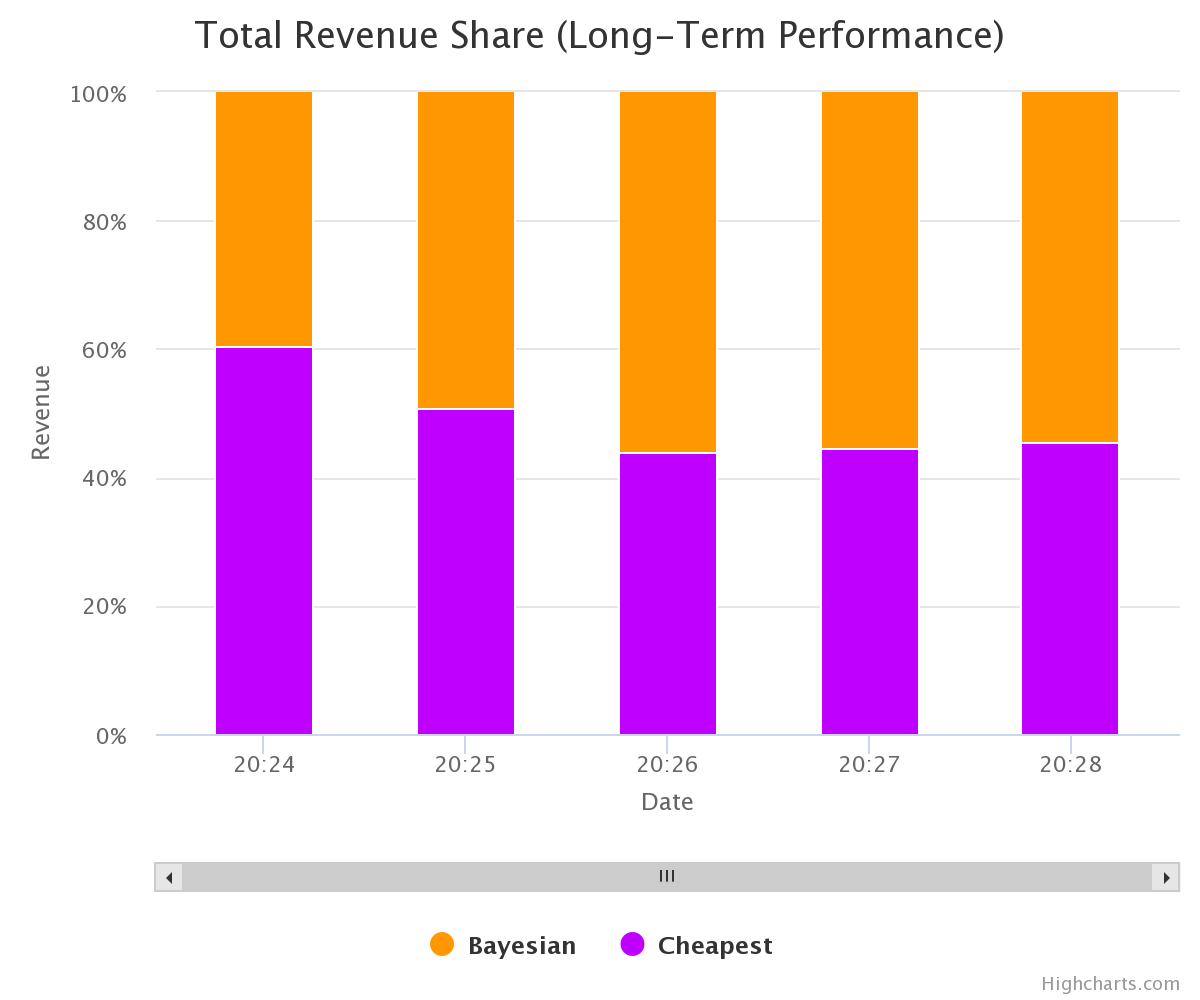
\includegraphics[width=\columnwidth]{pictures/lt_5.png}
  \caption{Long-Term Performance after 5 minutes}
  \label{fig:lt_5}
\end{figure}

This is the state after 5 minutes. The lead grows after half an hour and our merchant stabilizes at around 60\% market share (Appendix figure \ref{fig:lt_25}).

This result also shows in the revenue per hour chart (figure \ref{fig:rh_25}). The curve of our merchant rises faster than that of the cheapest merchant.

\begin{figure}[!htb]
  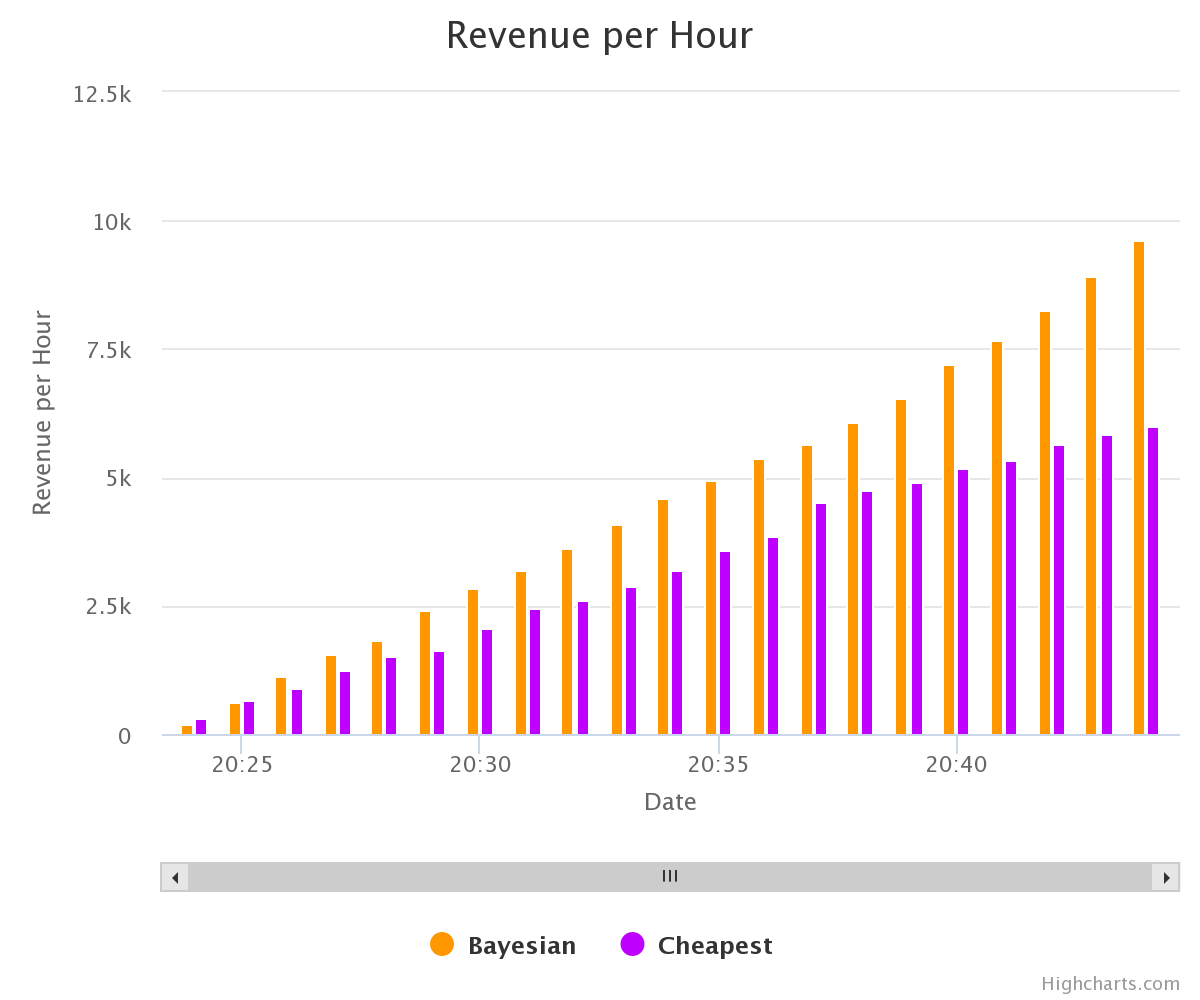
\includegraphics[width=\columnwidth]{pictures/rh_25.png}
  \caption{Revenue per hour after 30 minutes}
  \label{fig:rh_25}
\end{figure}

If we have a look at the price trajectory (figure \ref{fig:prices}), we can see that the merchant actually has a fairly aggressive behavior. At some points it sets very high prices. This seems to be a good strategy against the cheapest merchant. It probably tries to buy low-quality products to be able to sell them for little money. If a consumer wants to buy a high-quality product, they will have to buy it from our merchant, even though it is much more expensive than the products of the cheapest merchant.

\begin{figure}
  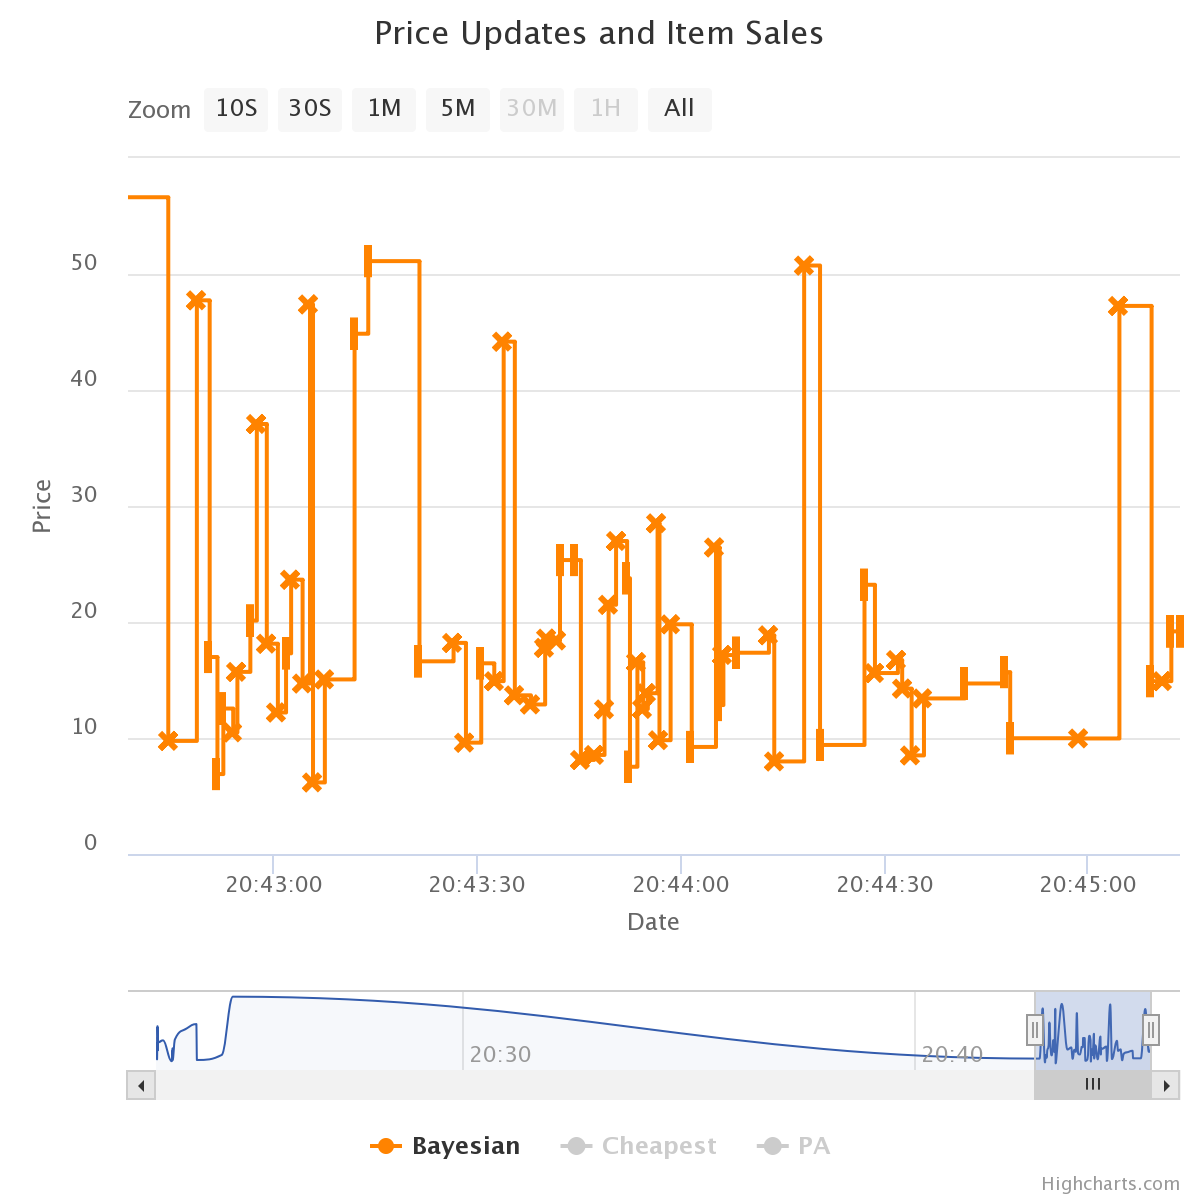
\includegraphics[width=\columnwidth]{pictures/prices.png}
  \caption{Price trajectory}
  \label{fig:prices}
\end{figure}

\section*{Conclusion}
While there are probably more sophisticated approaches out there, we showed that our simple solution was able to generate consistently profitable prices against an opponent that actually compromises its own profits in order to provide very cheap prices. With the help of automatized model generation and tuning we were able to beat this hostile behavior.\\
The scoring values of both approaches were not ideal, so there is the potential that more conservative machine learning or even deep learning approaches will get a better result, however it is always interesting to see how an supposed underdog compares to the favorites.

\newpage
\section*{Sources}
$^1$http://thestatsgeek.com/2014/02/08/r-squared-in-logistic-regression/\\
$^2$https://stats.stackexchange.com/questions/82105/mcfaddens-pseudo-r2-interpretation\\
$^3$http://scikit-learn.org/stable/modules/linear\_model.html\\
$^4$https://scikit-optimize.github.io/\\
$^5$https://en.wikipedia.org/wiki/Cross-validation\_(statistics)
\newpage
\section*{Appendix}
\begin{figure}[!htb]
  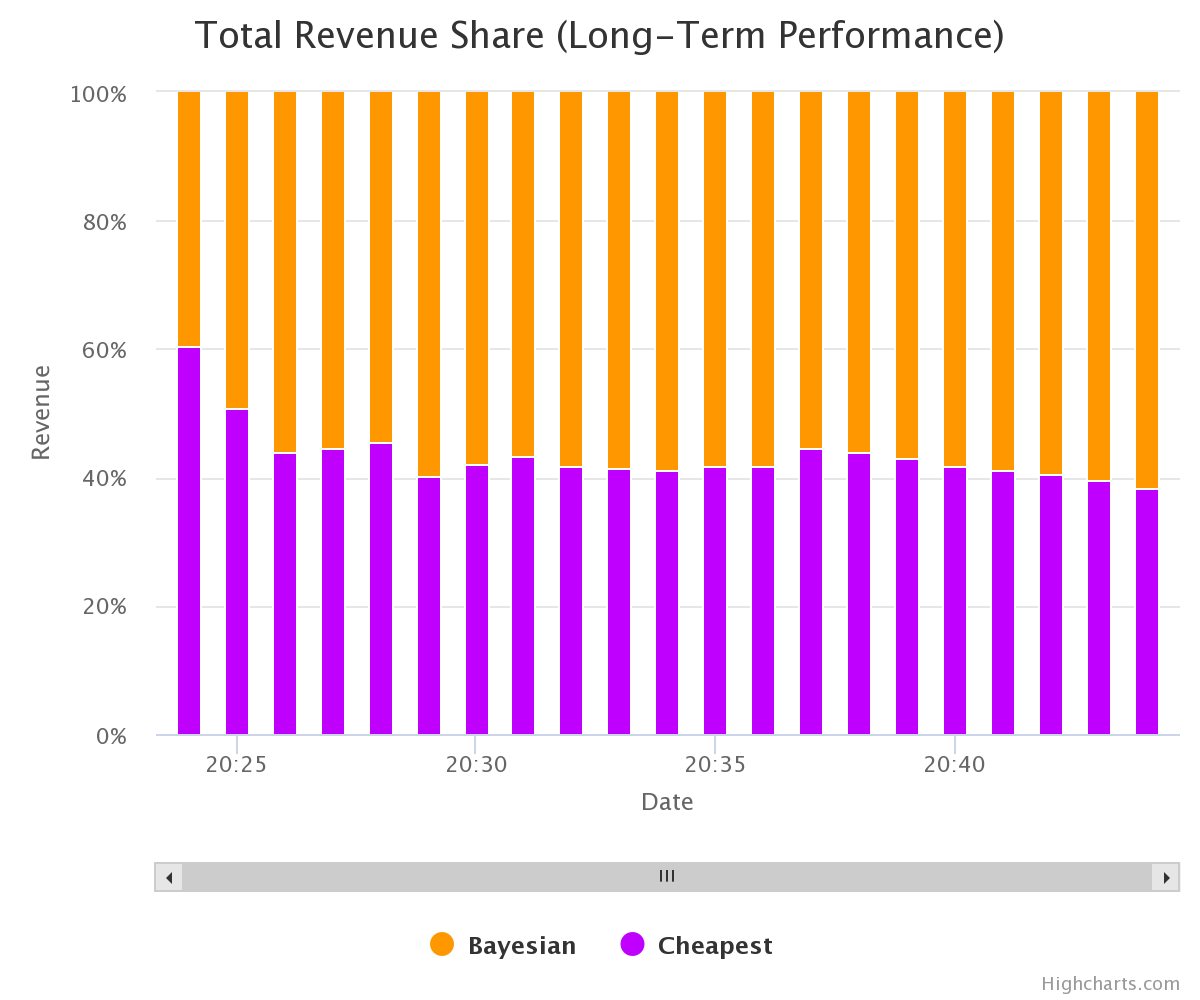
\includegraphics[width=\columnwidth]{pictures/lt_25.png}
  \caption{Long-Term Performance after 30 minutes}
  \label{fig:lt_25}
\end{figure}
\begin{figure}[!htb]
  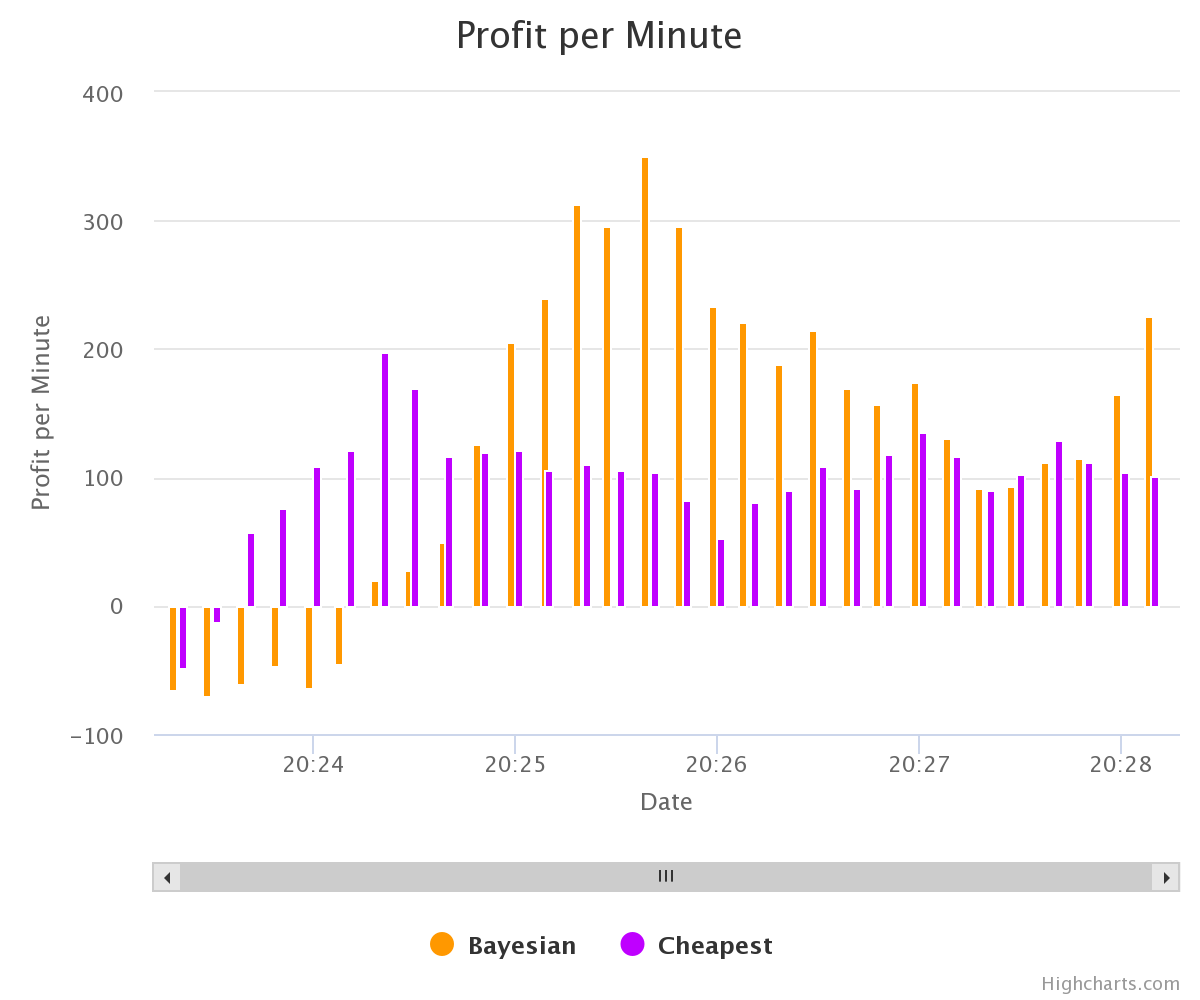
\includegraphics[width=\columnwidth]{pictures/ppm_5.png}
  \caption{Profit per minute after 5 minutes}
  \label{fig:ppm_5}
\end{figure}
\begin{figure}[!htb]
  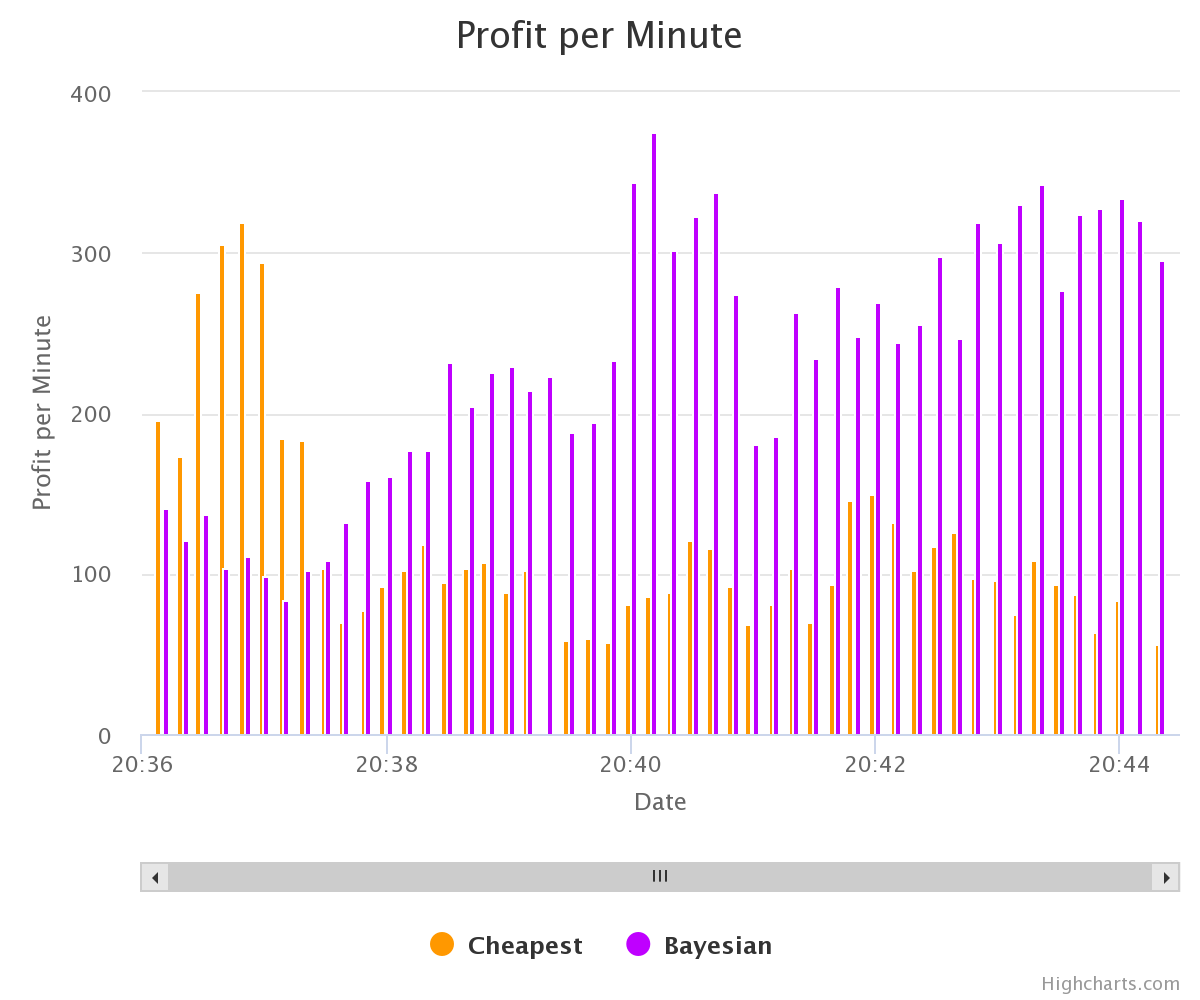
\includegraphics[width=\columnwidth]{pictures/ppm_25.png}
  \caption{Profit per minute after 30 minutes}
  \label{fig:ppm_25}
\end{figure}
\begin{figure}[!htb]
  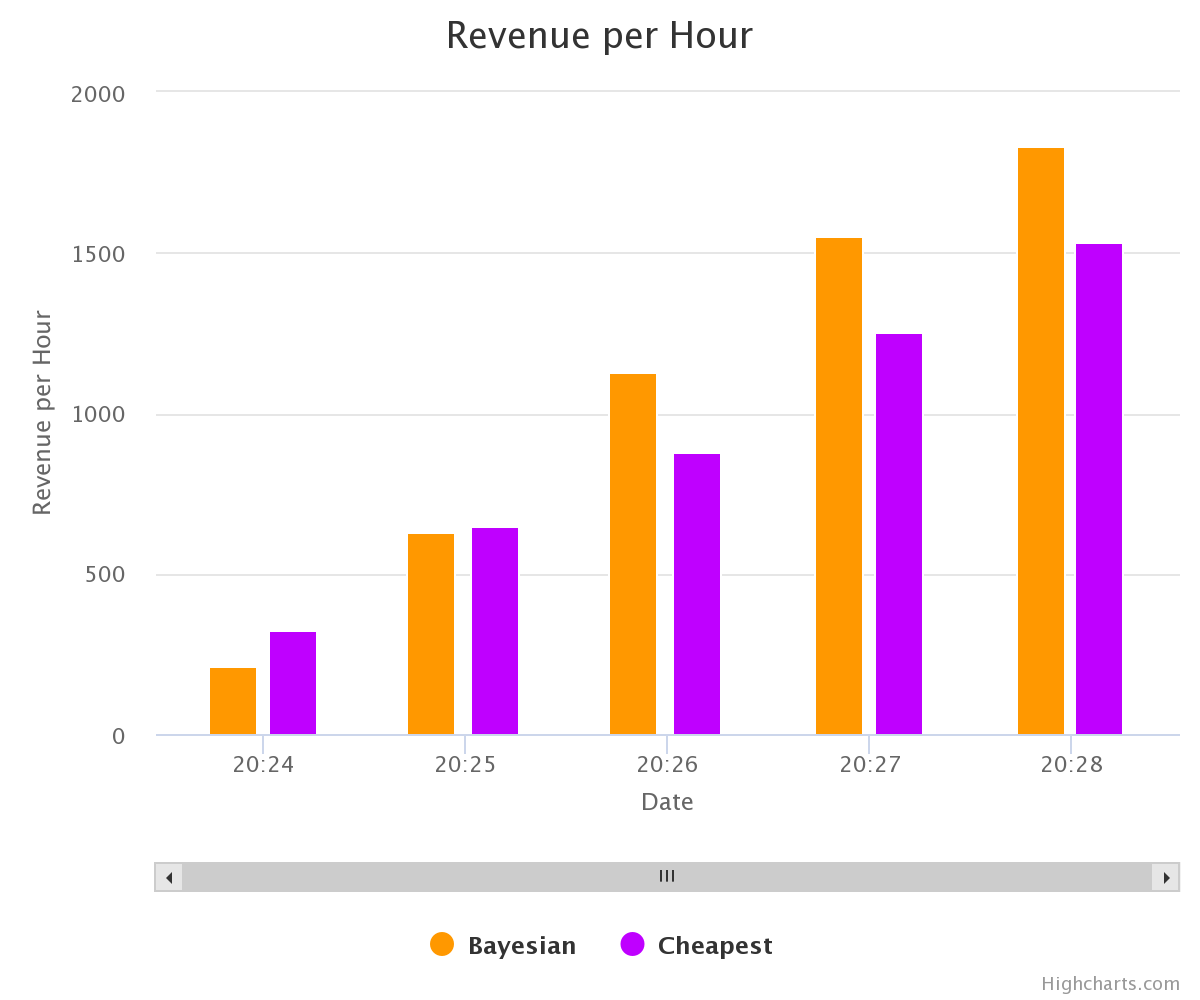
\includegraphics[width=\columnwidth]{pictures/rh_5.png}
  \caption{Revenue per hour after 5 minutes}
  \label{fig:rh_5}
\end{figure}
\begin{figure}[!htb]
  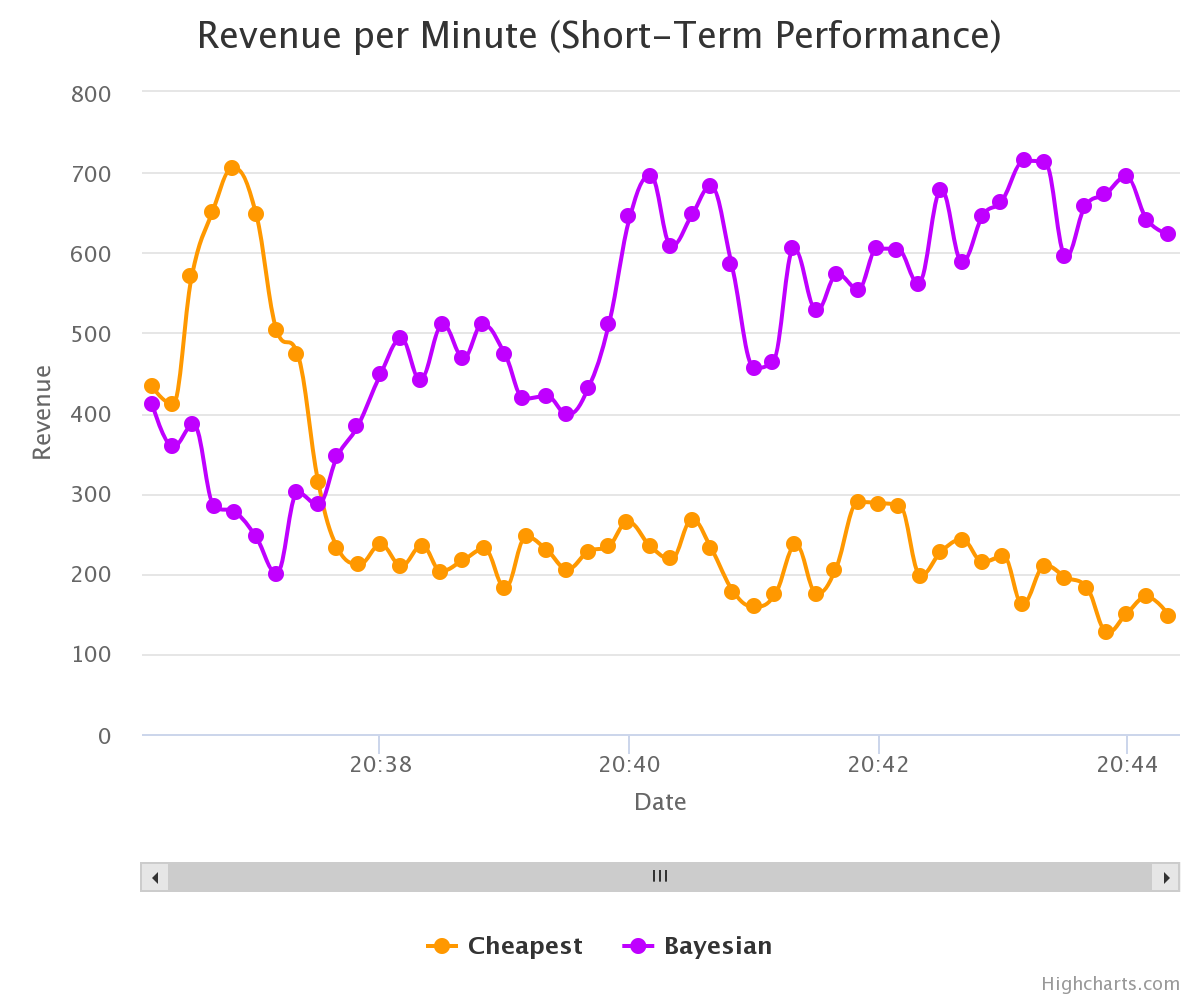
\includegraphics[width=\columnwidth]{pictures/st_25.png}
  \caption{Revenue per minute after 30 minutes}
  \label{fig:st_25}
\end{figure}
\end{document}
